% CVPR'27 submission — Learning Progress-Aware State Metrics (restructured draft)
% Compile: pdflatex main && bibtex main && pdflatex main && pdflatex main
\documentclass[10pt,twocolumn,letterpaper]{article}
\usepackage[review]{cvpr}
%% This file contains a number of tweaks that are typically applied to the main document.
%% They are not enabled by default, but can be enabled by uncommenting the relevant lines.


%%
%% Official support for 2-column teaser figure
%%
\usepackage{cuted} %< for strip environment

%%
%% For auto-referencing of figures (see fig/teaser.tex and \label{} therein) 
%%
\usepackage{currfile} %< for \currfilebase macro

%%
%% caption and (global) spacing overrides
%%
\usepackage{caption} %< for "\captionof" commands (teaser)
% \setlength{\abovecaptionskip}{.5em} % space above caption
% \setlength{\belowcaptionskip}{1em} % space below caption

%%
%% Inline annotations; for predefined colors, refer to "dvipsnames" in the xcolor package:
%% https://tinyurl.com/overleaf-colors
%%
\newcommand{\red}[1]{{\color{red}#1}}
\newcommand{\todo}[1]{{\color{red}#1}}
\newcommand{\TODO}[1]{\textbf{\color{red}[TODO: #1]}}
%%
%% Disable for camera ready / submission by uncommenting these lines:
%%
% \renewcommand{\TODO}[1]{}
% \renewcommand{\todo}[1]{#1}

%%
%% Work harder in optimizing text layout. Typically shrinks text by 1/6 of page, enable
%% it at the very end of the writing process, when you are just above the page limit.
%%
% \usepackage{microtype}

%%
%% Fine-tune paragraph spacing.
%%
% \renewcommand{\paragraph}[1]{\vspace{.5em}\noindent\textbf{#1.}}

%%
%% Globally adjusts space between figure and caption.
%%
% \setlength{\abovecaptionskip}{.5em}

%%
%% Allows "the use of \paper to refer to the project name"
%% with automatic management of space at the end of the word.
%%
% \usepackage{xspace}
% \newcommand{\paper}{ProjectName\xspace}

%%
%% Commonly used math definitions.
%%
% \DeclareMathOperator*{\argmin}{arg\,min}
% \DeclareMathOperator*{\argmax}{arg\,max}

%%
%% Tighten underline.
%%
% \usepackage{soul}
% \setuldepth{foobar}

%%
%% Reconfigure paragraph (tweaks spacing)
%%

\usepackage{booktabs}
\usepackage{multirow}
\usepackage{subcaption}
\usepackage{amsmath}
\usepackage{algorithm}
\usepackage{algpseudocode}
\usepackage{float}
\usepackage{xcolor}
\usepackage{xspace}

\newcommand{\method}{PABH\xspace}
\newcommand{\gtext}{\ensuremath{g_{\mathrm{text}}}}
\newcommand{\gset}{\ensuremath{g_{\mathrm{set}}}}
\newcommand{\Aepisode}{A^{\mathrm{ep}}}
\newcommand{\Astep}{A^{\mathrm{step}}}
\let\todo\undefined
\newcommand{\todo}[1]{\textcolor{red}{[TODO: #1]}}
\definecolor{cvprblue}{rgb}{0.21,0.49,0.74}
\usepackage[pagebackref,breaklinks,colorlinks,allcolors=cvprblue]{hyperref}

\def\confName{CVPR}
\def\confYear{2027}

\begin{document}
\raggedbottom
\title{Learning Progress-Aware State Metrics for Step-Level Credit\\Assignment in LLM Agents}
\author{Anonymous CVPR submission}
\maketitle

\begin{abstract}
Group-based reinforcement learning (RL) assigns credit to large language model (LLM) agent actions by comparing them with peer actions sampled under the same task. At the step level, this comparison is meaningful only when grouped states are comparable for credit assignment. Group-in-Group Policy Optimization (GiGPO) uses exact observation matches, whereas Bisimulation-Guided Policy Optimization with Action Counterfactual Estimation (BiPACE) clusters raw actor hidden states; neither explicitly addresses progress-confounded groups. We propose learning \emph{progress-aware state metrics} and instantiate them with \emph{progress-aware bisimulation heads} (\method). \method augments the anchor state with task-progress events and trains a lightweight linear projection with a Matching under Independent Couplings (MICo)-style objective anchored by rule-based process rewards. The learned embedding replaces raw hidden states for clustering, while counterfactual estimation, the policy prompt, extrinsic rewards, and the policy-optimization objective remain unchanged. Under our reproduction protocol, \method achieves the best overall results among the compared methods, reaching 95.1\% and 96.9\% success on ALFWorld and 74.2\% and 76.8\% success on WebShop at 1.5B and 7B, respectively. Component-attribution runs show that progress text alone is insufficient, while the trained head provides the main improvement. A retrospective analysis further shows that progress contamination can grow despite stable singleton coverage, motivating purity as a complementary diagnostic. These results support \method as a targeted mechanism for improving step-level credit where observation-based grouping confounds task progress.
\end{abstract}

\section{Introduction}
\label{sec:intro}

Long-horizon LLM agents must assign sparse terminal outcomes to intermediate decisions. Group-based policy optimization offers a critic-free alternative to learned value functions: GRPO and RLOO estimate relative advantages across sampled outputs~\cite{grpo,rloo,deepseek_r1}, and PPO provides the underlying policy-update machinery~\cite{ppo,sutton,gae}. Recent agent systems extend these ideas to multi-turn interactions~\cite{ragen,loop,archer}. GiGPO further constructs step-level groups by matching repeated observations across trajectories, adding local credit to the episode-level signal~\cite{gigpo}. BiPACE relaxes exact matching with actor-hidden clustering (BiGPO) and introduces action-conditioned counterfactual estimation (PACE)~\cite{bipace}.

These estimators share an implicit assumption: \emph{states placed in the same group must be comparable for credit assignment}. Exact observation identity can be too restrictive, but approximate grouping is not automatically better. The anchor observation often describes only the latest action feedback, so two states can look alike despite different completed subgoals and continuation values. Moreover, the actor hidden state is optimized for next-token prediction, not for value equivalence. Increasing group coverage can therefore reduce variance while introducing a more damaging bias: task progress is mistaken for action quality.

\begin{figure*}[t]
\centering
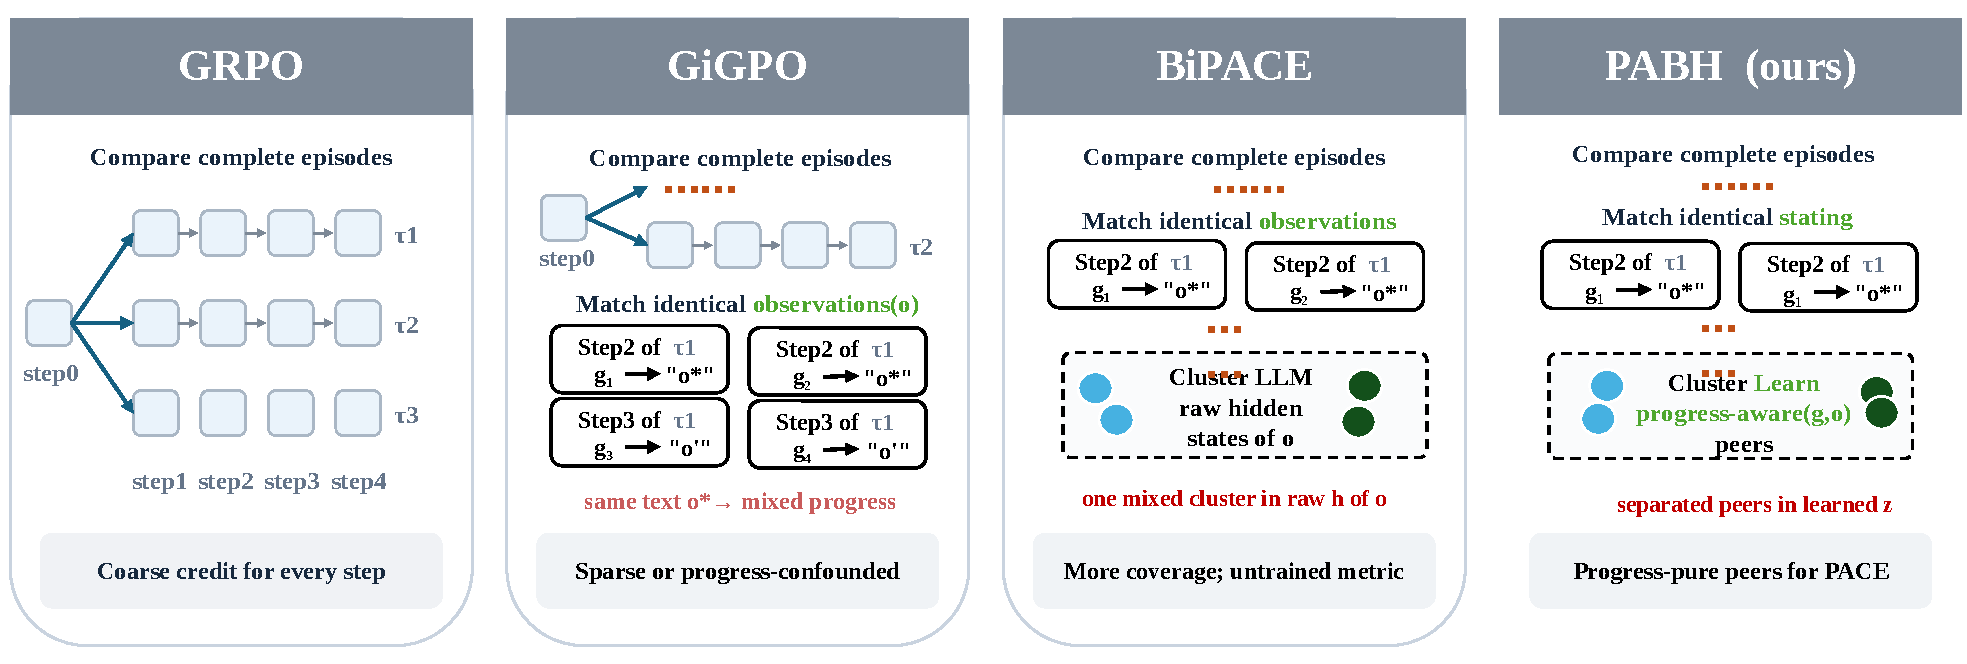
\includegraphics[width=\textwidth]{figs/fig_method_comparison.pdf}
\caption{Four ways to construct comparison units from the same rollout budget. GRPO compares complete episodes. GiGPO introduces step groups through exact observation matching, which can be sparse and progress-confused. BiPACE increases coverage using raw actor-hidden geometry, but its metric is not trained for value equivalence. \method augments the state with task progress and learns a bisimulation metric, producing cleaner peers for the inherited PACE estimator.}
\label{fig:comparison}
\end{figure*}

Figure~\ref{fig:comparison} contrasts these design choices. Our goal is not to maximize cluster size, but to form peer groups whose members are comparable in decision-relevant progress. We propose learning \emph{progress-aware state metrics} for step-level credit assignment and instantiate the metric with \emph{progress-aware bisimulation heads} (\method), comprising (i) a progress-event-augmented anchor state $s_t=(g_t,o_t)$, where $g_t$ summarizes task-relevant progress events; (ii) a linear projection trained online with a process-reward-anchored MICo objective; and (iii) the existing BiGPO--PACE consumption pipeline. The head reuses on-policy rollouts and adds only 0.39M/0.92M trainable parameters at 1.5B/7B. The policy prompt, extrinsic reward, and PPO objective are unchanged.

We evaluate the complete estimator ladder on ALFWorld and WebShop, using published GRPO references where available and same-pipeline reproductions for the principal step-level comparisons.

\begin{itemize}
\item \textbf{Progress-aware metric learning.} We combine explicit progress-event augmentation with a PRM-anchored bisimulation head, directly targeting value-equivalent state grouping without additional rollouts or changes to PPO rewards.
\item \textbf{Controlled evaluation across two environments.} We compare GiGPO, BiPACE-Q, and \method under a unified reproduction protocol, with published GRPO results as contextual references on ALFWorld and WebShop, reporting both improvements and regimes with limited additional benefit.
\item \textbf{Attribution and mechanism.} Mid-arm ablations separate progress-text injection from trained metric learning, while a retrospective analysis motivates group purity as a complementary diagnostic beyond singleton coverage.
\end{itemize}

\section{Related Work}
\label{sec:related}

\paragraph{Agentic reinforcement learning.}
Agentic RL extends policy optimization from single-turn responses to multi-turn environment interaction. ArCHer uses a hierarchical actor--critic decomposition for multi-turn agents~\cite{archer}; LoOP and RAGEN study optimization and training stability in long-horizon interactive settings~\cite{loop,ragen}; Search-R1 demonstrates outcome-based RL for multi-turn search agents~\cite{searchr1}. These works establish scalable agent-training pipelines, but terminal trajectory advantages alone cannot distinguish helpful from detrimental intermediate actions.

\paragraph{Group-based and step-level credit.}
PPO established clipped policy updates~\cite{ppo}, while GRPO and RLOO replace a learned critic with group-relative baselines~\cite{grpo,rloo}. GiGPO adds micro advantages by grouping repeated anchor states across trajectories~\cite{gigpo}. HGPO addresses inconsistent historical contexts with hierarchical grouping~\cite{hgpo}, while BiPACE replaces exact keys with actor-hidden clusters and action-conditioned PACE~\cite{bipace}. SALT instead derives step advantages from trajectory-graph structure~\cite{salt}. Our contribution is complementary to downstream credit estimators: we learn the state-equivalence metric that determines which steps should be compared.

\paragraph{Bisimulation and action-dependent credit.}
Bisimulation formalizes states with equivalent reward and transition behavior~\cite{givan,ferns}. DBC and MICo learn representations reflecting such behavioral distances~\cite{dbc,mico}. Our head adapts MICo-style pair fitting to a fixed late-layer LLM representation and replaces sparse terminal rewards with dense process anchors. We retain PACE as the downstream action-conditioned estimator and change only its input state metric.

\paragraph{Process supervision.}
PRMs and automatically constructed step supervision provide dense guidance in reasoning and agents~\cite{prm,mathshepherd,pqm,edu_prm,istar,turn_reward}. Instead of adding process rewards to the policy return, \method uses a deterministic progress signal only to train the state metric, leaving the PPO reward stream unchanged.

\section{Background: Group-Based Step Credit}
\label{sec:background}

For a prompt group $p$, GRPO samples $G$ trajectories $\{\tau^{(g)}\}_{g=1}^{G}$ under the same task prompt and normalizes their terminal returns to obtain an episode advantage $\Aepisode$. GiGPO adds a step term by grouping records with identical observations:
\begin{equation}
\Astep(i)=\frac{R_t^{(i)}-\mu_{C(i)}}{\sigma_{C(i)}+\delta},\qquad
A(i)=\Aepisode(i)+\omega\Astep(i),
\end{equation}
where $i$ indexes a step record at time $t$, $R_t^{(i)}$ is its discounted extrinsic return-to-go, and $C(i)$ is the anchor group containing $i$. The scalars $\mu_{C(i)}$ and $\sigma_{C(i)}$ are the group mean and standard deviation of $R_t$, $\delta>0$ prevents division by zero, and $\omega$ controls the step-advantage weight. Singleton groups provide no step-level signal.

BiPACE replaces the exact key with greedy cosine clustering over normalized actor hidden states $h_i$. Within each cluster, PACE estimates
\begin{equation}
\hat Q(s,a_i)=\operatorname{mean}_{j\in C^{=}(i)}R_t^{(j)},\quad
\hat V(s)=\operatorname{mean}_{j\in C(i)}R_t^{(j)},
\end{equation}
\begin{equation}
\Astep(i)=\hat Q(s,a_i)-\hat V(s),
\end{equation}
where $a_i$ is the action at record $i$, $C^{=}(i)=\{j\in C(i):a_j=a_i\}$ contains its same-action peers, $\hat Q(s,a_i)$ estimates the value of taking $a_i$ at the shared state $s$, and $\hat V(s)$ is the all-action cluster baseline. The estimator therefore depends on two choices: which states are comparable, and which action-conditioned returns are compared. \method changes only the first.

\section{Method}
\label{sec:method}

\subsection{Overview and a concrete failure case}
\method instantiates the proposed state metric with a lightweight linear bisimulation head. Figure~\ref{fig:pabh_method} illustrates the complete pipeline. At decision step $t$, $s_t$ denotes the environment state, $o_t$ the latest observation available to the agent, and $a_t$ the action sampled from the policy. A rollout record stores these quantities together with the subsequent observation and discounted return. We use $i$ and $j$ to index two records in the same on-policy prompt group. The actor is parameterized by $\theta$, and $\operatorname{Norm}(\cdot)$ denotes L2 normalization throughout. Consider two steps that both produce the feedback ``pick up kettle 1.'' Consider two steps that both produce the feedback ``pick up kettle 1.'' In one, the agent has only completed $\{\mathrm{take}(k_1)\}$; in the other, it has also completed $\{\mathrm{put}(k_2)\}$. The text feedback is identical, but the remaining task and continuation value differ. A raw observation or hidden-state group can mix these steps and attribute the later trajectory's advantage to the wrong action.

\begin{figure*}[t]
\centering
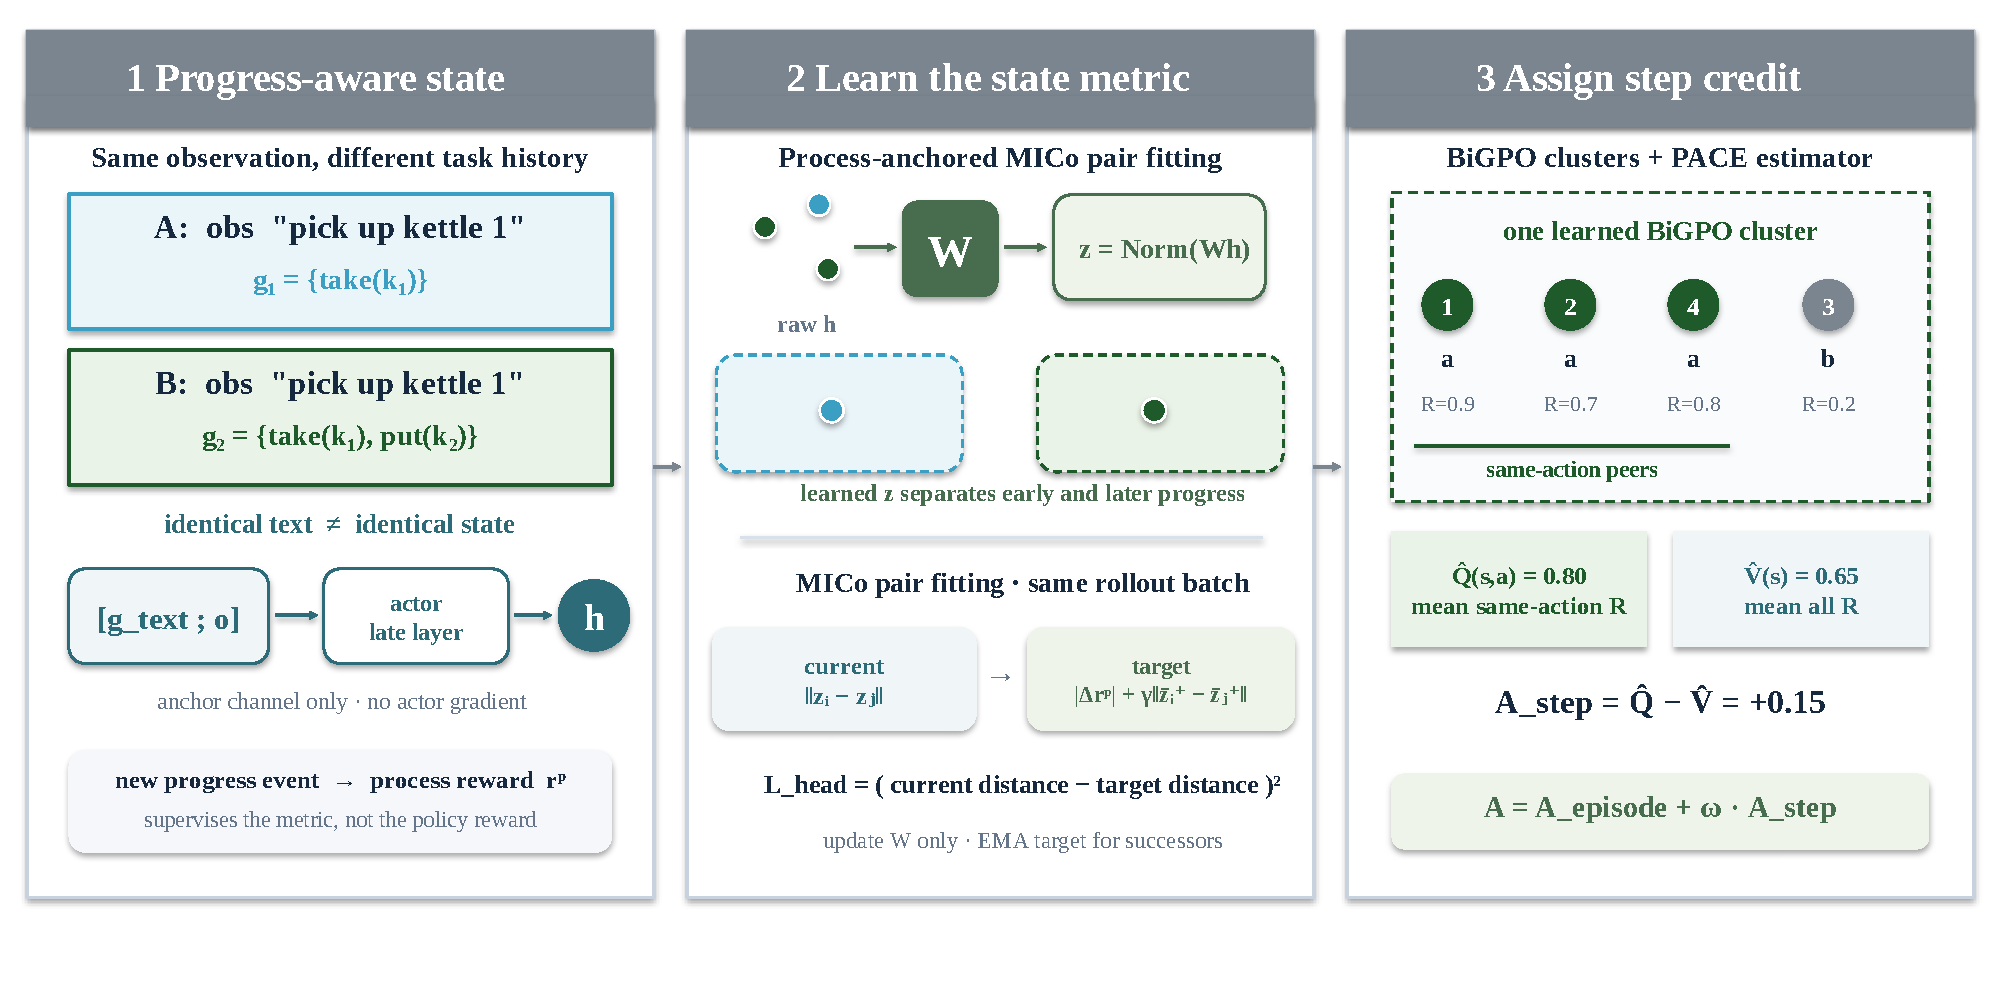
\includegraphics[width=\textwidth]{figs/fig_pabh_method.pdf}
\caption{\method overview with an illustrative ALFWorld-style example. Left: progress tracking distinguishes identical feedback by completed subgoals and constructs an anchor-only $[g_{\mathrm{text}};o]$ representation. Middle: a linear head learns $z=\mathrm{Norm}(Wh)$ by fitting current embedding distances to PRM differences plus discounted successor distances using an EMA target. Right: BiGPO forms clusters in $z$-space and PACE compares same-action and all-peer extrinsic returns. Numeric returns are illustrative: $\hat Q=0.80$, $\hat V=0.65$, and $\Astep=+0.15$. PRM shapes only the metric; PPO and its reward stream remain unchanged.}
\label{fig:pabh_method}
\end{figure*}

\subsection{Progress-grounded anchor states}
Let $g_t=g(s_t)$ denote a deterministic, environment-specific summary of task-relevant progress events available at state $s_t$. We maintain $g_t$ as an ordered event set $g_{\mathrm{set}}$ for contamination analysis and serialize it as $g_{\mathrm{text}}$ for representation learning. The anchor state is redefined as $(g_t,o_t)$, with progress text prepended only to the anchor observation:
\begin{equation}
\tilde o_t=[g_{\mathrm{text}};o_t],\qquad
h_t=\operatorname{Norm}\bigl(f_\theta(\tilde o_t)\bigr).
\end{equation}
Here $\tilde o_t$ is the progress-augmented anchor input, $f_\theta(\tilde o_t)\in\mathbb R^H$ is the actor's late-layer hidden vector at the last non-padding token, $H$ is its width, and $h_t$ is the normalized representation supplied to the metric head. The hidden vector is recomputed at advantage-computation time without an actor gradient. The policy prompt used to generate actions does not receive $g_{\mathrm{text}}$; progress injection affects the state metric, not the agent's input policy.

The progress representation is environment-specific but deterministic. ALFWorld uses anchored templates for six subgoal-event types and deliberately excludes navigation and container opening to avoid splitting states solely because of location changes. WebShop records search, item-view, and purchase events. Full serialization rules and anchor examples are given in Appendix~\ref{app:progress}.

\subsection{PRM-anchored bisimulation head}
A single bias-free linear projection $W\in\mathbb R^{256\times H}$ produces
\begin{equation}
z_t=\operatorname{Norm}(Wh_t).
\end{equation}
The projection acts as a low-rank Mahalanobis metric over the actor's nonlinear representation: $\|z_i-z_j\|_2^2=(h_i-h_j)^\top W^\top W(h_i-h_j)$ for normalized inputs. We use orthogonal initialization and L2-normalized outputs. Only $W$ receives the metric gradient; the actor is updated solely by the policy objective. An EMA target head $\bar W$, with the same shape as $W$, encodes successor states as $\bar z_t^{+}=\operatorname{Norm}(\bar Wh_{t+1})$.

For an on-policy pair $(i,j)$ sampled within a prompt group, let $r_i^p\in\mathbb R$ be a scalar process reward deterministically derived from the same progress events, and let $\bar z_i^{+}$ be the target-head embedding of $i$'s next anchor state. The discount $\gamma\in[0,1)$ balances immediate progress discrepancy against successor discrepancy. Both current states and successor states use the same progress augmentation. We fit
\begin{equation}
\mathcal L_{\mathrm{head}}=
\left(\|z_i-z_j\|_2-
\left[|r_i^p-r_j^p|+\gamma\|\bar z_i^{+}-\bar z_j^{+}\|_2\right]\right)^2.
\label{eq:mico}
\end{equation}
The target is detached, and $\bar W\leftarrow\tau W+(1-\tau)\bar W$ is applied after every head-gradient update, where $\tau\in(0,1)$ is the EMA update rate. Equation~\ref{eq:mico} encourages distances to track immediate progress differences and discounted behavioral divergence, rather than token-level surface similarity. Intuitively, two records become close when they have similar process rewards and their successor representations are close under the target metric; records with different completed subgoals remain separated even if their latest observations match. We resample 256 pairs per round, discard same-trajectory pairs closer than three steps to reduce trivial temporal correlations, and perform 30 head updates per PPO step.

The process reward is \emph{not} added to the environment return. It only supervises Eq.~\ref{eq:mico}; PACE and PPO continue to use extrinsic discounted returns.

\subsection{Clustering and action-conditioned consumption}
The learned $z_t$ replaces raw $h_t$ in BiGPO's prompt-group-local greedy cosine clustering. For a record embedding $z_i$ and cluster centroid $c$, $d_{\cos}(z_i,c)=1-z_i^\top c/\|z_i\|_2\|c\|_2$ is the cosine distance and $\varepsilon>0$ is the merge threshold. Records are processed within each prompt group: a record joins the nearest existing centroid when $d_{\cos}\leq\varepsilon$, otherwise it starts a new cluster. PACE then partitions each cluster by action identity, estimates $\hat Q$ from same-action peers and $\hat V$ from all peers, and computes $\Astep=\hat Q-\hat V$. The final advantage remains $A=\Aepisode+\omega\Astep$, where $\Aepisode$ supplies trajectory-level credit and $\Astep$ supplies local action credit.

Algorithm~\ref{alg:pabh_full} summarizes the complete pipeline. The projection used for the current advantage computation is produced before that step's head updates; updated weights affect subsequent steps. Actor parameters receive only the PPO gradient, while the head receives only the MICo gradient. Thus, our contribution is a drop-in state metric, not a second critic, a new rollout scheme, or a modified PPO surrogate.

\begin{algorithm*}[!t]
\caption{PABH training and advantage computation}
\label{alg:pabh_full}
\begin{algorithmic}[1]
\Require rollouts grouped by prompt, extrinsic rewards, progress trackers
\For{each PPO step}
  \State extract $g_t$, serialize $g_{\mathrm{text}}$, and form $\tilde o_t=[g_{\mathrm{text}};o_t]$ only for the anchor channel
  \State recompute $h_t=\mathrm{Norm}(f_\theta(\tilde o_t))$ at the last non-pad token without actor gradient
  \State $z_t\leftarrow\mathrm{Norm}(Wh_t)$ using the current head
  \For{$k=1$ to $10$}
    \State sample 256 on-policy pairs with valid next states; reject same-trajectory pairs with $|t_i-t_j|<3$
    \For{$u=1$ to $3$}
      \State update $W$ with $\mathcal L_{\mathrm{head}}$ from Eq.~\ref{eq:mico}
      \State $\bar W\leftarrow\tau W+(1-\tau)\bar W$
    \EndFor
  \EndFor
  \State cluster $\{z_t\}$ within each prompt group using greedy cosine clustering
  \State compute PACE $\Astep$ from extrinsic returns and $A=\Aepisode+\omega\Astep$
  \State update the actor with the unchanged PPO objective
\EndFor
\end{algorithmic}
\end{algorithm*}

\section{Experiments}
\label{sec:exp}

\subsection{Setup and evaluation protocol}
We evaluate ALFWorld~\cite{alfworld} and WebShop~\cite{webshop} with Qwen2.5-1.5B/7B-Instruct~\cite{qwen}. Our reproduced GiGPO, BiPACE-Q, and \method runs share the same rollout group size, environment configuration, training budget, and PPO implementation. BiPACE-Q and \method use the same official PACE convention within each environment and model scale (Appendix Table~\ref{tab:pace_config}).

\method uses a 256-dimensional head, learning rate $10^{-4}$, EMA rate $\tau=0.005$, and $\gamma=0.95$. The late layer is $-12$ for 1.5B and $-8$ for 7B; $\varepsilon$ follows the corresponding BiPACE configuration except on WebShop 1.5B, where BiPACE-Q uses 0.06 and \method uses 0.04, selected in an initial single-seed sweep before the remaining matched runs were completed. Training uses 200 PPO steps for 1.5B and 150 for 7B. Validation reports \emph{peak success within the stated budget}, averaged over the seeds shown in each cell.

All GiGPO, BiPACE-Q, and \method values in our experimental tables come from the same-pipeline reproductions. Prompt-only and ALFWorld/WebShop GRPO rows are published references used for context, not for controlled \method deltas. This preserves a direct check that training is beneficial while keeping comparisons among our principal RL methods consistent in code, hardware, prompts, and evaluation. Full configurations and per-seed ledgers appear in Appendices~\ref{app:hyperparams} and~\ref{app:per_seed}.

% CVPR'27 tables — published prompt-only/GRPO references + same-pipeline GiGPO/BiPACE-Q/PABH reproductions.

\begin{table*}[t]
\centering
\caption{Prompt-only references, published GRPO results, and same-pipeline GiGPO/BiPACE-Q/\method results on ALFWorld and WebShop. Prompt-only and GRPO rows reproduce BiPACE~\cite{bipace} and the results it cites, and are used for context rather than controlled \method deltas. GiGPO, BiPACE-Q, and \method rows are our reproductions. ALFWorld \emph{All} is count-weighted overall success. Per-task cells for our runs report complete readings at each run's overall-peak checkpoint; published GRPO cells retain their original protocol. WebShop Score and Success are independently maximized within budget. Parentheses show completed seeds.}
\label{tab:main}
\scriptsize
\setlength{\tabcolsep}{2.55pt}
\begin{tabular}{@{}llccccccccc@{}}
\toprule
& & \multicolumn{7}{c}{ALFWorld (valid-seen)} & \multicolumn{2}{c}{WebShop} \\
\cmidrule(lr){3-9}\cmidrule(l){10-11}
Model & Method & Pick & Look & Clean & Heat & Cool & Pick2 & All & Score & Succ. \\
\midrule
\multicolumn{11}{@{}l@{}}{\textit{Published prompt-only references (no fine-tuning; contextual comparison only).}} \\
\multicolumn{11}{@{}l@{}}{\textit{Closed-source models.}} \\
-- & GPT-4o & 75.3 & 60.8 & 31.2 & 56.7 & 21.6 & 49.8 & 48.0 & 31.8 & 23.7 \\
-- & Gemini-2.5-Pro & 92.8 & 63.3 & 62.1 & 69.0 & 26.6 & 58.7 & 60.3 & 42.5 & 35.9 \\
\midrule
\multicolumn{11}{@{}l@{}}{\textit{Qwen2.5-1.5B-Instruct.}} \\
1.5B & Qwen2.5 & 5.9 & 5.5 & 3.3 & 9.7 & 4.2 & 0.0 & 4.1 & 23.1 & 5.2 \\
1.5B & ReAct & 17.4 & 20.5 & 15.7 & 6.2 & 7.7 & 2.0 & 12.8 & 40.1 & 11.3 \\
1.5B & Reflexion & 35.3 & 22.2 & 21.7 & 13.6 & 19.4 & 3.7 & 21.8 & 55.8 & 21.9 \\
\midrule
\multicolumn{11}{@{}l@{}}{\textit{Published GRPO reference (training pipeline differs; contextual comparison only).}} \\
1.5B & GRPO & 85.3$\pm$1.5 & 53.7$\pm$8.0 & 84.5$\pm$6.8 & 78.2$\pm$7.9 & 59.7$\pm$5.0 & 53.5$\pm$5.6 & 75.2$\pm$3.8 & 75.8$\pm$3.5 & 56.8$\pm$3.8 \\
\midrule
\multicolumn{11}{@{}l@{}}{\textit{Qwen2.5-7B-Instruct.}} \\
7B & Qwen2.5 & 33.4 & 21.6 & 19.3 & 6.9 & 2.8 & 3.2 & 14.8 & 26.4 & 7.8 \\
7B & ReAct & 48.5 & 35.4 & 34.3 & 13.2 & 18.2 & 17.6 & 31.2 & 46.2 & 19.5 \\
7B & Reflexion & 62.0 & 41.6 & 44.9 & 30.9 & 36.3 & 23.8 & 42.7 & 58.1 & 28.8 \\
\midrule
\multicolumn{11}{@{}l@{}}{\textit{Published GRPO reference (training pipeline differs; contextual comparison only).}} \\
7B & GRPO & 90.8$\pm$5.1 & 66.1$\pm$6.7 & 89.3$\pm$5.4 & 74.7$\pm$6.9 & 72.5$\pm$5.4 & 64.7$\pm$7.3 & 77.6$\pm$5.2 & 79.3$\pm$2.8 & 66.1$\pm$3.7 \\
\midrule
\multicolumn{11}{@{}l@{}}{\textit{Same-pipeline RL training (GiGPO, BiPACE-Q, and \method; controlled comparisons use this block only).}} \\
\multicolumn{11}{@{}l@{}}{\textit{Qwen2.5-1.5B-Instruct.}} \\
1.5B & GiGPO
& \textbf{99.1$\pm$1.6} & 71.5$\pm$18.8 & 88.6$\pm$3.0 & \textbf{97.8$\pm$3.9} & 79.9$\pm$4.2 & 86.4$\pm$9.1
& 88.5$\pm$4.3 (3) & 86.3$\pm$1.3 (3) & 72.4$\pm$2.6 (3) \\
1.5B & BiPACE-Q
& 96.0$\pm$3.9 & 83.1$\pm$11.4 & \textbf{95.1$\pm$5.4} & 96.3$\pm$3.4 & 89.7$\pm$3.9 & \textbf{94.4$\pm$0.5}
& 92.7$\pm$3.0 (3) & 85.2$\pm$1.5 (3) & 69.8$\pm$1.6 (3) \\
1.5B & \method
& 96.6$\pm$1.4 & \textbf{88.4$\pm$11.1} & 93.6$\pm$2.3 & 95.0$\pm$8.7 & \textbf{100.0$\pm$0.0} & 92.1$\pm$3.4
& \textbf{95.1$\pm$1.8 (3)} & \textbf{88.6$\pm$1.7 (3)} & \textbf{74.2$\pm$4.8 (3)} \\
\midrule
\multicolumn{11}{@{}l@{}}{\textit{Qwen2.5-7B-Instruct.}} \\
7B & GiGPO
& 94.9$\pm$6.3 & 84.5$\pm$8.4 & 98.1$\pm$3.3 & 92.8$\pm$7.7 & 80.9$\pm$2.8 & 87.6$\pm$3.7
& 90.9$\pm$1.8 (3) & 86.2$\pm$1.1 (3) & 75.5$\pm$2.0 (3) \\
7B & BiPACE-Q
& \textbf{100.0$\pm$0.0} & 82.4$\pm$15.3 & 94.2$\pm$1.4 & \textbf{100.0$\pm$0.0} & 87.8$\pm$12.5 & \textbf{94.7$\pm$4.7}
& 94.0$\pm$1.6 (3) & 87.0$\pm$1.2 (3) & 73.1$\pm$0.6 (3) \\
7B & \method
& 98.8$\pm$2.1 & \textbf{90.4$\pm$4.9} & \textbf{100.0$\pm$0.0} & \textbf{100.0$\pm$0.0} & \textbf{96.8$\pm$5.5} & 93.0$\pm$3.3
& \textbf{96.9$\pm$1.6 (3)} & \textbf{88.1$\pm$0.7 (3)} & \textbf{76.8$\pm$0.8 (3)} \\
\bottomrule
\end{tabular}
\begin{flushleft}
\footnotesize Prompt-only and GRPO values and standard deviations are preserved from the cited sources. For our GiGPO, BiPACE-Q, and \method rows, we report the mean and sample standard deviation across completed seeds when at least two seeds are available, excluding post-budget checkpoints. For ALFWorld, all six task readings and the count-weighted \emph{All} score are taken from each run's overall-peak checkpoint. For WebShop, Score and Success are independently maximized within budget.
\end{flushleft}
\end{table*}


\subsection{Main results}
\label{sec:main}
Table~\ref{tab:main} compares the learned metric with published references and same-pipeline baselines. Prompt-only models provide a much lower reference point than trained agents in these settings, confirming that the observed gains cannot be attributed to prompting alone; published ALFWorld/WebShop GRPO rows provide an additional reference, while methodological comparisons involving \method use our same-pipeline GiGPO and BiPACE-Q results. On ALFWorld, where repeated feedback can hide different subgoal completion, \method obtains 95.1\% at 1.5B and 96.9\% at 7B, exceeding same-pipeline BiPACE-Q by 2.4 and 2.9 points, respectively. The reproduced GiGPO--BiPACE-Q--\method sequence further shows that approximate grouping, action-conditioned estimation, and metric training each contribute to the final estimator.

On WebShop, \method improves Success over BiPACE-Q by 4.4 points at 1.5B and 3.7 points at 7B. The dense Score metric also rises by 3.4 points at 1.5B (85.2 to 88.6) and by 1.1 points at 7B (87.0 to 88.1). With $\varepsilon=0.04$ and the same matched three-seed pool used by the other 1.5B methods, \method exceeds GiGPO in both Score (88.6 versus 86.3) and Success (74.2 versus 72.4). With $\varepsilon=0.05$, 7B \method likewise exceeds GiGPO in Score (88.1 versus 86.2) and Success (76.8 versus 75.5). WebShop therefore provides cross-scale evidence for the learned metric, although we retain the explicit $\varepsilon$ and initial single-seed selection protocol rather than treating these gains as universal across environments.

\subsection{Attribution: progress text versus trained metric}
\label{sec:attrib}
\begin{table}[htbp]
\centering
\caption{Progress-event and trained-head attribution on ALFWorld. ``$g_{\mathrm{text}}$ only'' uses the unprojected hidden state of the progress-augmented anchor without metric training. Parentheses show seed counts; these are component-attribution results rather than paired significance tests.}
\label{tab:attrib}
\small
\setlength{\tabcolsep}{5.0pt}
\begin{tabular}{@{}lcc@{}}
\toprule
Variant & 1.5B & 7B \\
\midrule
Raw (BiPACE-Q) & 92.7$\pm$3.0 (3) & 94.0$\pm$1.6 (3) \\
$g_{\mathrm{text}}$ only & 91.7$\pm$1.2 (3) & 95.1$\pm$1.2 (3) \\
$g_{\mathrm{text}}$ + \textbf{trained head} & \textbf{95.1$\pm$1.8 (3)} & \textbf{96.9$\pm$1.6 (3)} \\
\bottomrule
\end{tabular}
\end{table}
Table~\ref{tab:attrib} isolates the two additions on ALFWorld. At 1.5B, the completed mid-arm run reaches 91.7\%, below raw BiPACE-Q at 92.7\%, whereas the full method reaches 95.1\%. At 7B, the gains decompose more evenly: 94.0\% with raw anchors, 95.1\% with progress text only, and 96.9\% with the trained head.

The mid-arm and full arms have different completed seed counts, so we interpret this as component attribution rather than a paired statistical test. The evidence suggests that $g_{\mathrm{text}}$ is an enabler that exposes progress to the representation, while the trained metric is the principal source of improvement at 1.5B. Simply adding text is insufficient in these experiments; learning how to organize that information is important.

\subsection{Mechanism: purity rather than coverage}
\label{sec:purity}
We retrospectively reconstruct exact-observation groups from 15 completed ALFWorld runs spanning raw-anchor, progress-text, and head variants, and measure singleton coverage together with cluster- and pair-level progress contamination. As shown in Fig.~\ref{fig:purity}, singleton coverage stays flat near $1.5\%$ over training, while pair-level contamination grows. Stable coverage can therefore conceal increasingly progress-inconsistent comparisons.

\begin{figure}[htbp]
\centering
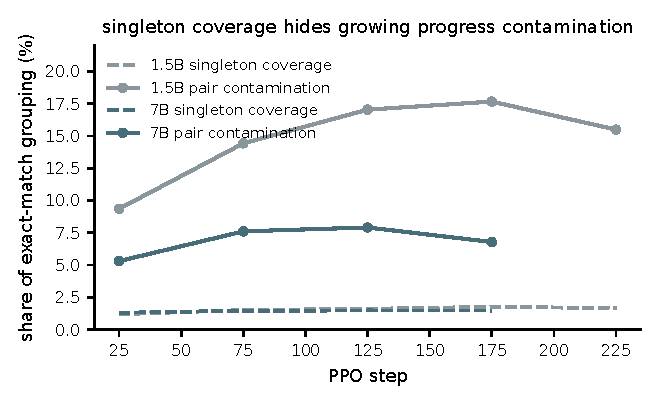
\includegraphics[width=\linewidth]{figs/fig_purity.pdf}
\caption{Retrospective progress-contamination analysis on 15 completed ALFWorld runs spanning raw-anchor, progress-text, and head variants. Singleton exact-match coverage (dashed) stays flat near $1.5\%$ over training, while pair-level progress contamination (solid) grows. These are descriptive diagnostics of exact-observation grouping across training variants, not direct evaluations of learned-$z$ clusters or causal purity--success estimates.}
\label{fig:purity}
\end{figure}

Coverage and contamination capture distinct failure modes. Singleton records fall back to episode credit, whereas contaminated groups can bias action credit; neither statistic is a universal stand-alone quality metric. The appropriate goal is to improve peer comparability rather than merely reduce singletons. Metric definitions are provided in Appendix~\ref{app:purity}. This retrospective analysis motivates purity as a complementary diagnostic, but does not directly compare raw-$h$ and learned-$z$ clusters or establish a purity--success relationship.

\subsection{Efficiency and limitations}
\method adds 0.39M/0.92M trainable parameters at 1.5B/7B and no extra rollouts or learned critic. The head consumes the same rollout batch and accounts for less than 2\% of training-step time in our measurements. The linear head is a simplicity and efficiency choice rather than a demonstrated optimum over nonlinear alternatives. Nevertheless, progress extraction requires environment-specific rules or dense scores, limiting direct application to open-ended feedback without reliable progress detectors. The current trackers are heuristic event summaries rather than complete state reconstructions, so richer goal-conditioned serialization may further improve the metric. Several estimator cells still require additional seeds, and peak validation can be sensitive to isolated spikes. Finally, our current comparison focuses on the GRPO--GiGPO--BiPACE ladder; graph-based credit consumers such as G2PO are complementary directions rather than same-pipeline baselines in this draft.

\section{Conclusion}
We presented a framework for learning progress-aware state metrics, instantiated by \method, a lightweight bisimulation head for step-level credit assignment in LLM agents. By combining explicit progress-event summaries with PRM-anchored metric learning, \method improves the state equivalence used by BiGPO and PACE while preserving the rollout budget, PPO reward, and policy objective. Same-pipeline results across ALFWorld and WebShop show the benefits of trained progress-aware grouping across both benchmarks. The central lesson is that step-level credit depends not merely on how many states are grouped, but on whether those states should be compared at all.

{\small
\bibliographystyle{ieeenat_fullname}
\bibliography{refs}
}

\appendix
% Appendix for PABH: implementation, diagnostics, per-seed results, and reproducibility.

\section{Implementation Details}
\label{app:algorithm}

The head is a bias-free linear map $W\in\mathbb R^{256\times H}$ with orthogonal initialization and L2-normalized outputs. Its parameter count is $256H$: 393,216 for $H=1536$ (1.5B) and 917,504 for $H=3584$ (7B). The EMA target head is initialized as a copy of $W$, has \texttt{requires\_grad=False}, and is checkpointed together with the online head and its optimizer. Pair endpoints must have valid same-trajectory successors. Sampling uses a fixed local RNG, and successor targets are detached.

The anchor forward pass is separate from rollout generation. It disables the language-model head, reads the selected late layer, and applies no gradient to the actor. Head optimization runs on the driver CPU; the same rollout batch supplies current and successor hidden states, process rewards, and extrinsic returns.

\section{Progress Extraction and Anchor Serialization}
\label{app:progress}

Table~\ref{tab:progress_rules} gives the environment-specific progress contract. Progress text is prepended only to the metric anchor; the policy prompt retains its original history and observation. An empty progress history produces no text prefix.

\begin{table}[!b]
\centering
\caption{Progress-event and process-reward specifications. Process rewards are consumed only by the MICo loss.}
\label{tab:progress_rules}
\scriptsize
\renewcommand{\arraystretch}{1.12}
\begin{tabular}{@{}p{1.65cm}p{5.55cm}@{}}
\toprule
Environment & Specification \\
\midrule
ALFWorld & \textbf{Events.} Ordered, deduplicated $(\mathrm{predicate},\mathrm{object})$ events: take, clean, cool, heat, put, toggle. Object IDs are retained; receptacles are discarded except that toggle uses the receptacle as its event object. Navigation, open/close, look, and inventory are excluded. \\
& \textbf{Example.} \texttt{[Progress] completed subgoals:\newline take(egg 3), heat(egg 3)} \\
& \textbf{PRM.} $+1$ win; $+0.5$ per new progress event; $-0.1$ for ``Nothing happens.''; $0$ otherwise. \\
\midrule
WebShop & \textbf{Events.} Search-action count, viewed-item events, and purchase outcome. Navigation clicks and item subpages are excluded from the set. \\
& \textbf{Example.} \texttt{[Progress] searches issued: 2;\newline items viewed: item A, item B} \\
& \textbf{PRM.} $+1$ correct purchase; $-0.5$ wrong purchase; $+0.2$ per new item view; $-0.1$ invalid action; $0$ otherwise. \\
\bottomrule
\end{tabular}
\end{table}

For ALFWorld, the six anchored templates are:
\texttt{pick up}, \texttt{clean}, \texttt{cool}, \texttt{heat}, \texttt{move}, and \texttt{turn on}. Only the first observation line is matched, preventing task instructions or history from creating false events. Navigation and container opening are intentionally excluded because they need not change task completion, although this is an approximation rather than a full MDP-state equivalence guarantee.

Across environments, the progress text is an environment-specific event summary rather than a complete MDP-state reconstruction. It supplies deterministic task-relevant side information beyond the latest observation, but does not by itself certify bisimulation equivalence. Designing richer goal-conditioned serializers is a promising direction for future work.

A representative anchor input is therefore:
\begin{quote}\small
\texttt{[Progress] completed subgoals: take(kettle 1)}\newline
\texttt{You pick up the kettle 1 from the stoveburner 1.}
\end{quote}
The corresponding policy prompt contains only the usual task history and observation, not the bracketed progress prefix.

\section{Hyperparameters and Evaluation Protocol}
\label{app:hyperparams}

\noindent\begin{minipage}{\columnwidth}
\centering
\captionof{table}{Shared head-training settings. Values are taken from the adopted run scripts, not library defaults.}
\label{tab:head_hparams}
\small
\renewcommand{\arraystretch}{1.15}
\begin{tabular}{@{}p{3.8cm}p{3.7cm}@{}}
\toprule
Setting & Adopted value \\
\midrule
Projection dim. / init & 256 / orthogonal \\
Head learning rate & $10^{-4}$ \\
EMA rate $\tau$ & 0.005 / update \\
MICo discount $\gamma$ & 0.95 \\
Pairs per round & 256 (replacement) \\
Rounds $\times$ updates & $10\times3=30$ / PPO step \\
Same-trajectory min. $\Delta t$ & 3 \\
Target & EMA (detached) \\
Head optimizer / device & Adam / driver CPU \\
\bottomrule
\end{tabular}
\end{minipage}

\begin{table}[h]
\centering
\caption{Environment- and scale-specific clustering and PACE configuration. A single $\varepsilon$ is shared; two values denote BiPACE-Q/\method.}
\label{tab:pace_config}
\scriptsize
\renewcommand{\arraystretch}{1.12}
\setlength{\tabcolsep}{1.5pt}
\begin{tabular}{@{}lcccc@{}}
\toprule
Setting & A-1.5B & A-7B & W-1.5B & W-7B \\
\midrule
$\varepsilon$ (Q/\method) & 0.05 & 0.10 & 0.06/0.04 & 0.08/0.05 \\
Layer & $-12$ & $-8$ & $-12$ & $-8$ \\
Rollout group & 8 & 8 & 12 & 12 \\
Action key & first-8 & action-tag & action-tag & action-tag \\
PACE estimator & counterfactual & Q-style & Q-style & Q-style \\
PPO steps & 200 & 150 & 200 & 150 \\
\bottomrule
\end{tabular}
\begin{flushleft}
\scriptsize A = ALFWorld; W = WebShop. first-8 = first 8 response tokens; action-tag = \texttt{<action>} body. BiPACE-Q and \method share the action key and estimator within each column.
\end{flushleft}
\end{table}

For WebShop 1.5B, \method's $\varepsilon=0.04$ was selected in an initial single-seed sweep; two additional runs were then completed to form the same matched three-seed pool used by GiGPO and BiPACE-Q. For WebShop 7B, \method's $\varepsilon=0.05$ was selected in an initial single-seed sweep before two additional runs were completed; the current BiPACE-Q row retains $\varepsilon=0.08$ while its 0.10 refresh remains in progress.

All reproductions use NVIDIA H20 nodes, with four GPUs per run except the official two-GPU WebShop 1.5B protocol. The actor learning rate is $5\times10^{-7}$, the return discount is 0.95, the step-advantage weight is 1.0, and the invalid-action penalty is 0.1. Validation runs every ten PPO steps. ALFWorld uses 128 valid-seen episodes with temperature 0.4.

ALFWorld \emph{All} is the count-weighted success at each run's overall-peak checkpoint; per-task values are read at that same checkpoint rather than independently maximized. WebShop Score and Success are independently maximized within budget. Post-budget checkpoints are excluded. We use logged peaks from all resume segments rather than \texttt{best\_checkpoint.txt}, which can omit peaks before a restart.

\section{Purity and Coverage Diagnostics}
\label{app:purity}

The retrospective analysis reconstructs exact-observation groups within each prompt group and recomputes $g_{\mathrm{set}}$ using the same progress tracker as training. Let $\mathcal{C}$ be the set of exact-observation clusters with $|C|>1$, and let $g_i$ denote the progress set of record $i$. We define
\begingroup
\setlength{\abovedisplayskip}{5pt}
\setlength{\belowdisplayskip}{5pt}
\begin{align}
\operatorname{conf}_{\mathrm{clus}} &=
\frac{\#\{C\in\mathcal{C}:\exists i,j\in C,\ g_i\neq g_j\}}
{|\mathcal{C}|}, \label{eq:conf_clus}\\
\operatorname{conf}_{\mathrm{pair}} &=
\frac{\sum_{C\in\mathcal{C}}\#\{\{i,j\}\subset C:g_i\neq g_j\}}
{\sum_{C\in\mathcal{C}}\binom{|C|}{2}}. \label{eq:conf_pair}
\end{align}
\endgroup
The first statistic is the fraction of clusters containing records with different progress sets; the second is the fraction of progress-inconsistent record pairs. The exact-match singleton rate is the fraction of one-record groups. Purity, the complement of contamination, is used as a qualitative diagnostic rather than a new advantage estimator.

\section{Reproducibility and Cost Checks}
\label{app:repro}

Our implementation checks the following invariants: (i) $g_{\mathrm{text}}$ never enters the policy prompt; (ii) process rewards have no consumer in the PPO return path; (iii) the actor receives no MICo gradient; and (iv) PACE consumes extrinsic discounted returns.

The only trainable additional parameters are the $256H$ projection weights. \method requires no additional environment rollouts or learned critic. It does require an anchor forward pass, pair sampling, 30 CPU head updates per PPO step, and clustering. Prompt-only and ALFWorld/WebShop GRPO table rows are published references. All GiGPO, BiPACE-Q, and \method values, as well as every \method delta, come from our same-pipeline reproductions.

\section{Full Per-Seed Results and Run Ledger}
\label{app:per_seed}

For seed pools larger than three, we report three runs from a matched pool shared across methods rather than selecting by outcome. Other completed runs remain in the experiment logs but are not used in these aggregates. When overall peaks tie, we use the earliest peak checkpoint for every per-task reading.

\begin{table}[h]
\centering
\caption{ALFWorld per-seed overall peak success (\%). Slash-separated values show individual runs in each reported pool.}
\label{tab:alf_seeds}
\scriptsize
\renewcommand{\arraystretch}{1.15}
\setlength{\tabcolsep}{2.5pt}
\begin{tabular}{@{}llp{3.4cm}r@{}}
\toprule
Model & Method & Per-seed peak values & Mean$\pm$std \\
\midrule
1.5B & GRPO & Published aggregate & 75.2$\pm$3.8 \\
1.5B & GiGPO & 83.6 / 90.6 / 91.4 & 88.5$\pm$4.3 (3) \\
1.5B & BiPACE-Q & 90.6 / 91.4 / 96.1 & 92.7$\pm$3.0 (3) \\
1.5B & \method & 93.0 / 96.1 / 96.1 & 95.1$\pm$1.8 (3) \\
\midrule
7B & GRPO & Published aggregate & 77.6$\pm$5.2 \\
7B & GiGPO & 89.8 / 93.0 / 89.8 & 90.9$\pm$1.8 (3) \\
7B & BiPACE-Q & 92.2 / 95.3 / 94.5 & 94.0$\pm$1.6 (3) \\
7B & \method & 96.9 / 98.4 / 95.3 & 96.9$\pm$1.6 (3) \\
\bottomrule
\end{tabular}
\begin{flushleft}
\scriptsize GRPO rows are published aggregates, not from our run ledger. ALFWorld 1.5B BiPACE-Q uses the first-$n$ + counterfactual protocol.
\end{flushleft}
\end{table}

\begin{table}[h]
\centering
\caption{WebShop per-seed Score and Success at 1.5B (\%). Each metric is independently maximized within budget.}
\label{tab:webshop_seeds}
\scriptsize
\renewcommand{\arraystretch}{1.15}
\setlength{\tabcolsep}{1.0pt}
\begin{tabular}{@{}llp{2.8cm}r@{}}
\toprule
Method & Metric & Per-run values & Mean$\pm$std \\
\midrule
GRPO & Score & Published aggregate & 75.8$\pm$3.5 \\
 & Success & Published aggregate & 56.8$\pm$3.8 \\
\midrule
GiGPO & Score & 84.9 / 87.3 / 86.8 & 86.3$\pm$1.3 \\
 & Success & 69.9 / 75.0 / 72.3 & 72.4$\pm$2.6 \\
\midrule
BiPACE-Q & Score & 84.0 / 86.8 / 84.7 & 85.2$\pm$1.5 \\
 & Success & 70.3 / 71.1 / 68.0 & 69.8$\pm$1.6 \\
\midrule
\method & Score & 88.2 / 87.1 / 90.4 & 88.6$\pm$1.7 \\
 & Success & 77.7 / 68.8 / 76.2 & 74.2$\pm$4.8 \\
\bottomrule
\end{tabular}
\end{table}

\begin{table}[!t]
\centering
\caption{WebShop per-seed Score and Success at 7B (\%). Each metric is independently maximized within budget.}
\label{tab:webshop_seeds_7b}
\scriptsize
\renewcommand{\arraystretch}{1.15}
\setlength{\tabcolsep}{1.0pt}
\begin{tabular}{@{}llp{2.8cm}r@{}}
\toprule
Method & Metric & Per-run values & Mean$\pm$std \\
\midrule
GRPO & Score & Published aggregate & 79.3$\pm$2.8 \\
 & Success & Published aggregate & 66.1$\pm$3.7 \\
\midrule
GiGPO & Score & 85.9 / 85.2 / 87.4 & 86.2$\pm$1.1 \\
 & Success & 75.0 / 73.8 / 77.7 & 75.5$\pm$2.0 \\
\midrule
BiPACE-Q & Score & 85.7 / 87.8 / 87.6 & 87.0$\pm$1.2 \\
 & Success & 72.7 / 73.8 / 72.7 & 73.1$\pm$0.6 \\
\midrule
\method & Score & 87.6 / 88.9 / 87.8 & 88.1$\pm$0.7 \\
 & Success & 76.6 / 76.2 / 77.7 & 76.8$\pm$0.8 \\
\bottomrule
\end{tabular}
\begin{flushleft}
\scriptsize GRPO rows are published aggregates, not from our run ledger. \method uses $\varepsilon=0.04$ at 1.5B and $\varepsilon=0.05$ at 7B.
\end{flushleft}
\end{table}


\end{document}
